\section{Ejercicio 1}

Se deseo diseñar un filtro notch pasivo con $f_0$ = $18.9 kHz$ para el siguiente circuito: 

\begin{figure}[h]
	\centering
	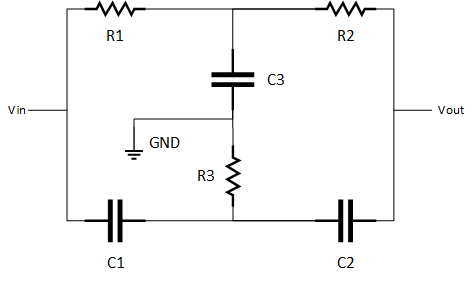
\includegraphics[scale=1]{../EJ1/circuito.png}
	\caption{Filtro Notch Pasivo}
	\label{ej1cir}
\end{figure}

La determinación de los valores de las resistencias y capacitores requieren primeramente la función de trasferencia del circuito, es decir que se deberá hallar una resolución del circuito. Para ello tomaremos las siguientes direcciones de corriente, de las cuales obtenemos las siguientes ecuaciones:

\begin{wrapfigure}{l}{0.5\textwidth}
\centering
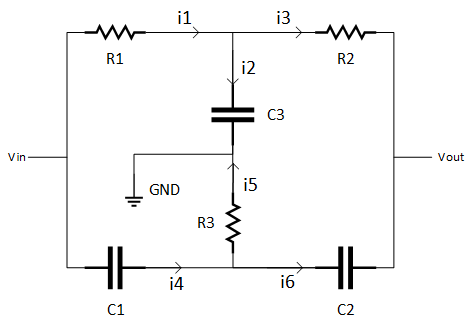
\includegraphics[scale=0.6]{../EJ1/circuitois.png}
\caption{Flujo de Corrientes}
\label{fig_2}
\end{wrapfigure}


$$Vin = R_1 .i_1 + X_{C3}.i_2 \hspace{1cm} Vout = -R_2 .i_3 + X_{C3}.i_2$$
$$Vin = R_3 .i_5 + X_{C2}.i_4 \hspace{1cm} Vout = R_3 .i_5 - X_{C2}.i_2$$

Como sabemos que $i_1 = i_2 + i_3$, $i_4 = i_5 + i_6$ y $i_6 = - i_3$ podemos analizar las ecuaciones algebraicamente resultando en:

$$i_2 (R_1 + 2.X_{C3}) = i_5 (2.R_3+X_{C1}) + i_3 (X_{C2} - X_{C1})$$

Al considerar $R = R1 = R2 = 2 \cdot R3$ y $C = C1 = C2 = \frac{C3}{2}$ 
$$\therefore i_2 = i_5$$

Por lo que la función de transferencia sera igual a:

$$\frac{Vout}{Vin} = \frac{X_C^2 + R^2}{R^2 + 4RX_c + X_C^2} \hspace{0.5cm}\Rightarrow \hspace{0.5cm} H(s) = \frac{s^2C^2R^2 + 1}{s^2R^2C^2 + s4RC + 1}$$




